\documentclass[xcolor=dvipsnames,professionalfonts,smaller,presentation]{beamer} 
\usecolortheme[named=Brown]{structure} 
\useoutertheme{miniframes}
\usetheme{Malmoe}
\usepackage{graphicx}
\usepackage{verbatim}
\usepackage[portuguese]{babel}
\usepackage[latin1]{inputenc}
\usepackage{alltt}
\usepackage{moreverb}
\usepackage{hyperref}
\usepackage{indentfirst}
\usepackage{lastpage}
\usepackage{array}
\usepackage{url}
\usepackage{float}
\usepackage{subfigure}
\usepackage{multirow}

\urldef{\mails}\path|ei05011@fe.up.pt,ei05028@fe.up.pt|
\title[Classification on the Adult Database \insertframenumber/\inserttotalframenumber]{A comparison of classification algorithms applied to the Adult Database}
\author{Fl�vio Cruz and Jo�o Azevedo}
\institute{Faculdade de Engenharia da Universidade do Porto\\
\mails}
\date{\today}

\begin{document}

\frame{\titlepage}

\section[Outline]{}
\frame{\tableofcontents}

\section{Problem proposed by the Dataset}
\frame
{
    \frametitle{Problem proposed by the Dataset}

    \begin{itemize}
    \item Given an adult with some attributes, identify whether he gains more than 50000 dollars per year, or not.
    \item Identify what social characteristics allow one person to gain more than someone else.
    \item Understanding what affects the income can give a lot of information concerning society's behaviour.
    \end{itemize}
}

\section{Dataset Characterization}

\subsection{The Dataset}
\frame
{
    \frametitle{The Dataset}
    
    \begin{itemize}
    \item 48842 entries of individual information of people gathered in a 1994 census on the United States of America.
    \begin{itemize}
        \item 32561 records for the training set (67\%).
        \item 16281 records for the test set (33\%).
    \end{itemize}
    \item Each entry is composed by a set of 14 attributes and 2 classes (winning more or less than 50K dollars a year).
    \item There are 3620 records with missing values. The only attributes containing missing values are \textbf{Workclass}, \textbf{Occupation} and \textbf{Native-country}.
    \item Available in \url{ftp://ftp.ics.uci.edu/pub/machine-learning-databases/adult}.
    \end{itemize}
}

\frame
{
    \frametitle{Attributes}

    \begin{itemize}
        \item \textbf{Age} (continuous).
        \item \textbf{Workclass} (categorical).
        \item \textbf{FNLWGT} (continuous).
        \item \textbf{Education} (ordinal).
        \item \textbf{Education-num} (continuous).
        \item \textbf{Marital-status} (categorical).
        \item \textbf{Occupation} (categorical).
        \item \textbf{Relationship} (categorical).
        \item \textbf{Race} (categorical).
        \item \textbf{Sex} (categorical).
        \item \textbf{Capital-gain} (continuous).
        \item \textbf{Capital-loss} (continuous).
        \item \textbf{Hours-per-week} (continuous).
        \item \textbf{Native country} (categorical).
    \end{itemize}   
}

\subsection{Data Analysis}
\frame
{
    \frametitle{Value distribution in the training set}

\footnotesize
\begin{table}
\subtable[Age]{
       \begin{tabular}{| l | l |}
       \hline
       Min. & 17 \\
       \hline
       1st Qu. & 28 \\
       \hline
       Median & 37 \\
       \hline
       Mean & 38.58 \\
       \hline
       3rd Qu. & 48 \\
       \hline
       Max & 90 \\
       \hline
       \end{tabular}
}
\qquad\qquad
\subtable[Workclass]{        
       \begin{tabular}{| l | l |}
       \hline
       private & 22696 \\
       \hline
       self\_emp\_not\_inc & 2541 \\
       \hline
       local\_gov & 2093 \\
       \hline
       state\_gov & 1298 \\
       \hline
       self\_emp\_inc & 1116 \\
       \hline
       (Other) & 981 \\
       \hline
       NA's & 1836 \\
       \hline
       \end{tabular}
}
\qquad\qquad
\subtable[Education]{        
       \begin{tabular}{| l | l |}
       \hline
       hs\_grad & 10501 \\
       \hline
       some\_college & 7291 \\
       \hline
       bachelors & 5535 \\
       \hline
       masters & 1723 \\
       \hline
       assoc\_voc & 1382 \\
       \hline
       11th & 1175 \\
       \hline
       (Other) & 5134 \\
       \hline
       \end{tabular}
}
\qquad\qquad
\subtable[Marital Status]{        
       \begin{tabular}{| l | l |}
       \hline
       divorced & 4443 \\
       \hline
       married\_af\_spouse & 23 \\
       \hline
       married\_civ\_spouse & 14976 \\
       \hline
       married\_spouse\_absent & 418 \\
       \hline
       never\_married & 10683 \\
       \hline
       separated & 1025 \\
       \hline
       widowed & 993 \\
       \hline
       \end{tabular}
}
\end{table}
\normalsize
}

\frame
{
    \frametitle{Value distribution in the training set}

\footnotesize
\begin{table}
\subtable[Occupation]{        
       \begin{tabular}{| l | l |}
       \hline
       prof\_specialty & 4140 \\
       \hline
       craft\_repair & 4099 \\
       \hline
       exec\_managerial & 4066 \\
       \hline
       adm\_clerical & 3770 \\
       \hline
       sales & 3650 \\
       \hline
       (Other) & 10993 \\
       \hline
       NA's & 1843 \\
       \hline
       \end{tabular}
}
\qquad\qquad
\subtable[Relatonship]{        
       \begin{tabular}{| l | l |}
       \hline
       husband & 13193 \\
       \hline
       not\_in\_family & 8305 \\
       \hline
       other\_relative & 981 \\
       \hline
       own\_child & 5068 \\
       \hline
       unmarried & 3446 \\
       \hline
       wife & 1568 \\
       \hline
       \end{tabular}
}
\qquad\qquad
\subtable[Race]{        
       \begin{tabular}{| l | l |}
       \hline
       amer\_indian\_eskimo & 311 \\
       \hline
       asian\_pac\_islander & 1039 \\
       \hline
       black & 3124 \\
       \hline
       other & 271 \\
       \hline
       white & 27816 \\
       \hline
       \end{tabular}
}
\qquad\qquad
\subtable[Sex]{        
       \begin{tabular}{| l | l |}
       \hline
       female & 10771 \\
       \hline
       male & 21790 \\
       \hline
       \end{tabular}
}
\end{table}
\normalsize
}

\frame
{
    \frametitle{Value distribution in the training set}

\footnotesize
\begin{table}
\subtable[Capital Gain]{        
       \begin{tabular}{| l | l |}
       \hline
       Min. & 0 \\
       \hline
       1st Qu. & 0 \\
       \hline
       Median & 0 \\
       \hline
       Mean & 1078 \\
       \hline
       3rd Qu. & 0 \\
       \hline
       Max. & 99999 \\
       \hline
       \end{tabular}
}
\qquad\qquad
\subtable[Capital Loss]{        
       \begin{tabular}{| l | l |}
       \hline
       Min. & 0 \\
       \hline
       1st Qu. & 0 \\
       \hline
       Median & 0 \\
       \hline
       Mean & 87.3 \\
       \hline
       3rd Qu. & 0 \\
       \hline
       Max. & 4356 \\
       \hline
       \end{tabular}
}
\qquad\qquad
\subtable[Hours Per Week]{        
       \begin{tabular}{| l | l |}
       \hline
       Min. & 1 \\
       \hline
       1st Qu. & 40 \\
       \hline
       Median & 40 \\
       \hline
       Mean & 40.44 \\
       \hline
       3rd Qu. & 45 \\
       \hline
       Max. & 99 \\
       \hline
       \end{tabular}
}
\qquad\qquad
\subtable[Native Country]{        
       \begin{tabular}{| l | l |}
       \hline
       United States & 29170 \\
       \hline
       Mexico & 643 \\
       \hline
       Philippines & 198 \\
       \hline
       Germany & 137 \\
       \hline
       Canada & 121 \\
       \hline
       (Other) & 1709 \\
       \hline
       NA's & 583 \\
       \hline
       \end{tabular}
}
\qquad\qquad
\subtable[Plus 50]{        
       \begin{tabular}{| l | l |}
       \hline
       No & 24720 \\
       \hline
       Yes & 7841 \\
       \hline
       \end{tabular}
}
\end{table}
\normalsize
}

\frame
{
    \frametitle{Some obvious relationships}
    
    \begin{itemize}
    \item There is a higher percentage of older people gaining more than 50K than younger ones.
    \item There is a higher percentage of people with more education gaining more than 50K than people with less studies.
    \item There is a higher percentage of workaholics gaining more than 50K than people who work in part-time.
    \end{itemize}

   \begin{minipage}{0.30\linewidth}
        \begin{figure}
        \centering
            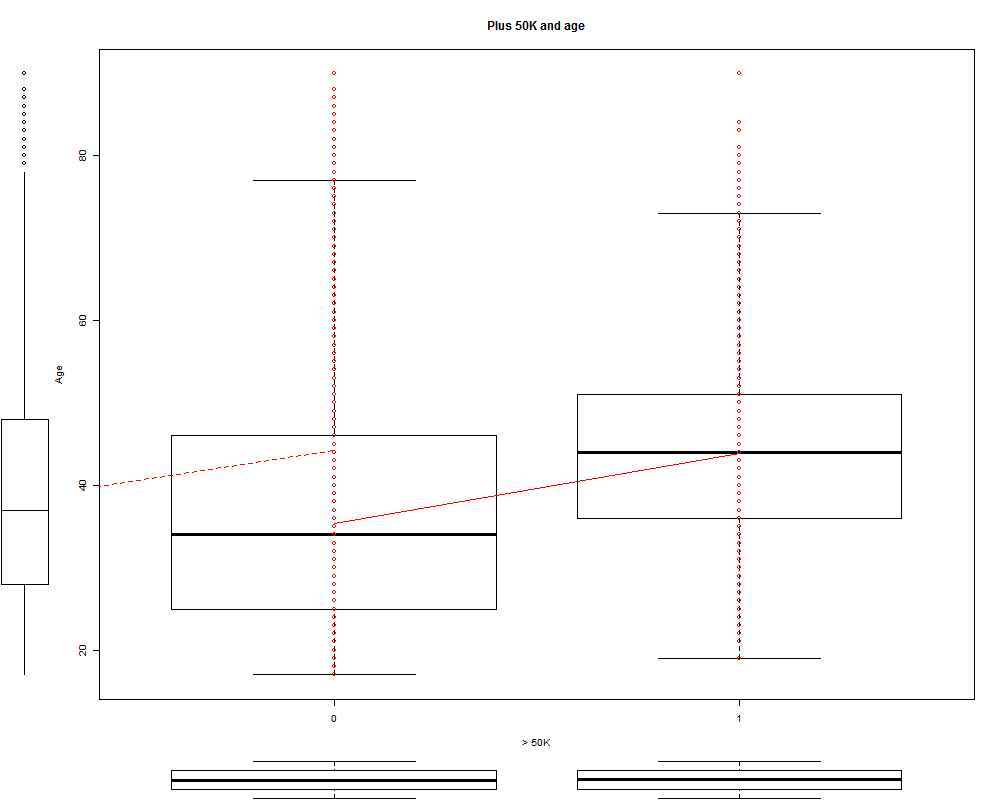
\includegraphics[width=3.5cm]{plot_plus_50_age.png}
        \end{figure}
    \end{minipage}
    \hspace{0.1cm}
    \begin{minipage}{0.30\linewidth}
        \begin{figure}
        \centering
            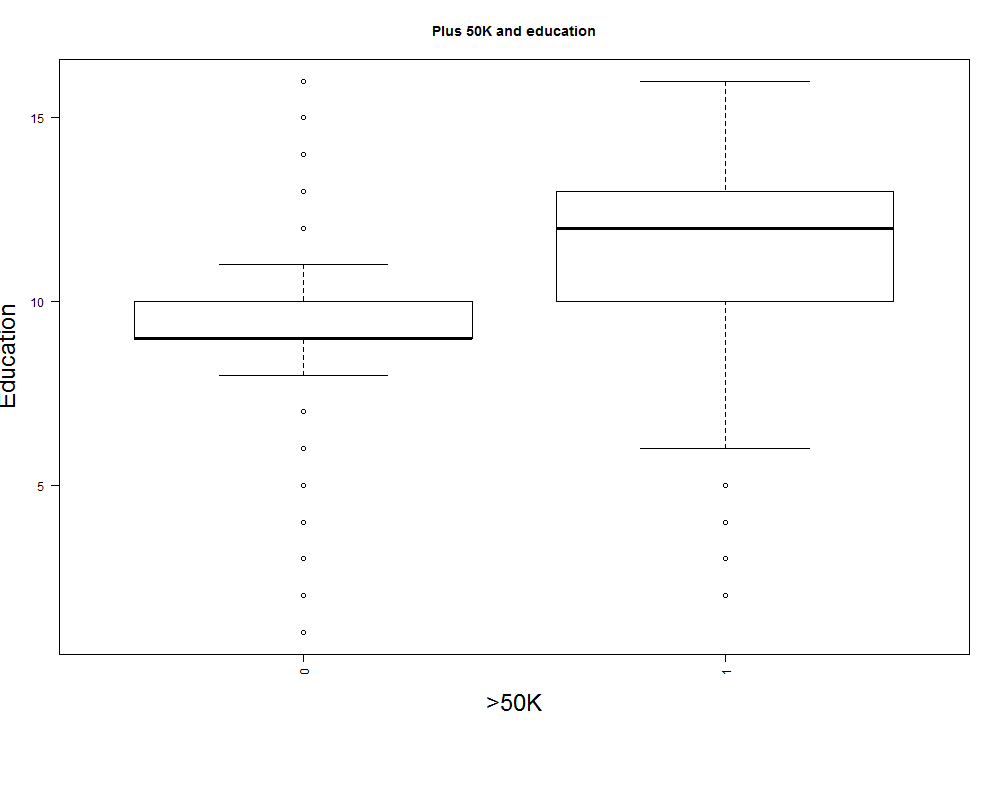
\includegraphics[width=3.5cm]{plot_plus_50_education_num.png}
        \end{figure}
    \end{minipage}
    \hspace{0.1cm}
    \begin{minipage}{0.30\linewidth}
        \begin{figure}
        \centering
            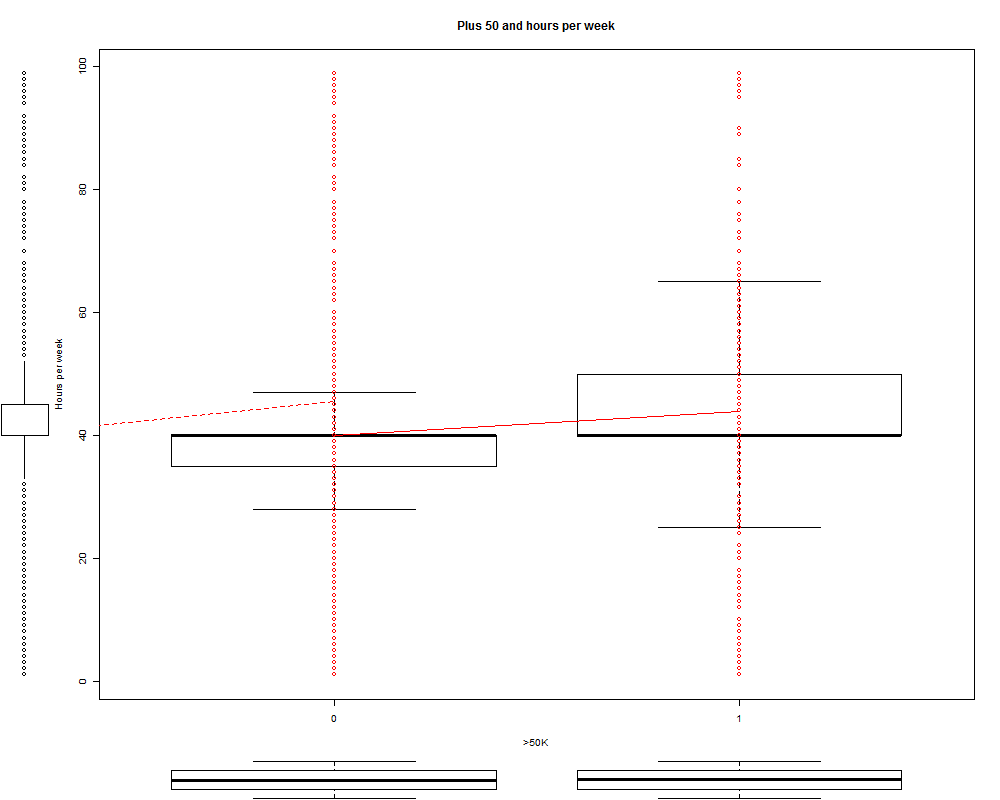
\includegraphics[width=3.5cm]{plot_plus_50_hpw.png}
        \end{figure}
    \end{minipage}
}

\frame
{
    \frametitle{Association Rules}
    
    \begin{itemize}
      \item  Association rules can be used to discover interesting relations and patterns between attributes.
     
    \end{itemize}
    
    \begin{table}[ht]
        \begin{center}
        \scalebox{1.0}{
          
        \begin{tabular}{ | m{5cm} | c | c | c | }
        \hline
        \textbf{Rule / LHS} & \textbf{RHS} & \textbf{Support} & \textbf{Confidence} \\ \hline
        \footnotesize{age=young, hours\_per\_week=part\_time}�& $<$50K & 0.05730782 & 1 \\ \hline
        \footnotesize{marital\_status=never\_married, relationship=own\_child, hours\_per\_week=part\_time} & $<$50K & 0.04689659 & 1 \\ \hline
        \footnotesize{age=young, relationship=own\_child, hours\_per\_week=part\_time} & $<$50K & 0.04404042 & 1 \\ \hline
        \footnotesize{relationship=husband, capital\_gain=high} & $>$50K & 0.02251159 & 0.9918809 \\ \hline
        \footnotesize{relationship=husband, race=white, sex=male, capital\_gain=high} & $>$50K & 0.02063819 & 0.9926145 \\ \hline
        \end{tabular}}
        \label{tbl:arules_income}
        \end{center}
    \end{table}
}

\frame
{
    \frametitle{Clusters}

    \begin{itemize}
    \item Clustering can be used to detect similar individuals and to build classes in the absence of them.
    \item Generating 6 clusters with only three variables (\textbf{age}, \textbf{education\_num} and \textbf{hours\_per\_week}) leads to some interesting observations:
    \begin{itemize}
        \item Younger people are grouped together.
        \item People with different levels of education belong to different clusters.
    \end{itemize}
    \end{itemize}
}

\section{Data Mining Problem}
\frame
{
    \frametitle{Data Mining Problem}

    \begin{itemize}
    \item The database poses a classification problem.
    \item There is no single classifier that works best on all given problems:
    \begin{itemize}
        \item Decision trees.
        \item Rule induction.
        \item Inductive logic programming.
        \item Bayesian classifiers.
    \end{itemize}
    \end{itemize}
}

\section{Algorithms Used}
\frame
{
  \frametitle{Algorithms Used}
  
  \begin{itemize}
    \item Decision trees
    
    \begin{itemize}
      \item ID3
      \item C4.5
      \item CART
      \item Random Forest
      \item Alternating Decision Trees (ADTree)
    \end{itemize}
    
    \item Rule Induction
    
    \begin{itemize}
      \item  CN2
    \end{itemize}
    
    \item Inductive Logic Programming
    \begin{itemize}
        \item Aleph
    \end{itemize}
    
    \item Bayesian Networks. Using different search algorithms:
    
    \begin{itemize}
      \item Genetic Search
      \item Hill Climbing
      \item Simulated Annealing
    \end{itemize}
    
  \end{itemize}
}

\section{Conducted Experiments}
\frame
{
  \frametitle{Conducted Experiments}
  
  \begin{itemize}
    \item Classifiers were built using the train set and then tested against the test set
    \item C4.5, Random Forest, CART, ADTree and Bayesian classifiers built using Weka
    \begin{itemize}
      \item Various parameters available in Weka algorithms were experimented in hope of getting better error rates
      \item Every missing value was replaced with modes and means
      \item Two different classifiers were trained for each algorithm, one using only discretized attributes
                and another with the attributes unmodified
      \item Analyze how the algorithm behaves when using numeric attributes
    \end{itemize}
  \end{itemize}
}

\frame
{
  \frametitle{Conducted Experiments}

  \begin{itemize}
    \item RapidMiner was used to build a classifier with the ID3 algorithm.
    \item Peter Clark's CN2 was used to induce rules.
    \begin{itemize}
        \item \url{http://www.cs.utexas.edu/users/pclark/software/\#cn2}.
    \end{itemize}
    \item Aleph was used to inductively generate logic clauses.
    \begin{itemize}
        \item \url{http://www.comlab.ox.ac.uk/activities/machinelearning/Aleph/aleph.html}.
    \end{itemize}
  \end{itemize}
}

\subsection{ID3}
\frame
{
    \frametitle{ID3}

    \begin{itemize}
        \item ID3 in RapidMiner is implemented in two different flavours: one that supports numerical values, one that doesn't.
        \item An absolute discretization was conducted on numerical values for the version that doesn't support them.
        \item RapidMiner supports different splitting criterions: Gain Ratio, Information Gain, Gini Index or Accuracy.
    \end{itemize}

\footnotesize
\begin{table}[ht]
  \begin{center}
  \begin{tabular}{ | l | c | c | c | c | c |}
    \hline
    \textbf{Type} & \textbf{Criterion} & \textbf{Train error rate} & \textbf{Test error rate} & \textbf{Time} \\ \hline
    ID3 & Gain Ratio & 18.38 & 18.61 & 0m04s \\ \hline
    ID3 & Information Gain & 18.48 & 19.05 & 0m03s \\ \hline
    ID3 & Gini Index & 18.94 & 19.15 & 0m04s \\ \hline
    ID3 & Accuracy & 20.41 & 20.24 & 0m04s \\ \hline
    ID3 Numerical & Gain Ratio & 14.93 & 15.68 & 0m14s \\ \hline
    ID3 Numerical & Information Gain & 15.68 & 16.42 & 0m06s \\ \hline
    ID3 Numerical & Gini Index & 16.10 & 16.96 & 0m07s \\ \hline
    ID3 Numerical & Accuracy & 17.99 & 17.92 & 0m12s \\ \hline
  \end{tabular}
  \end{center}
\end{table}
\normalsize
}

\subsection{C4.5}
\frame
{
  \frametitle{C4.5}
  
  \begin{itemize}
    \item Weka supports a confidence threshold parameter that dictates how much pruning the algorithm will do
    \item The bigger the threshold the less pruning the algorithm does
    \item When using only discretized data the algorithm gives error rates of $\approx$25\%
  \end{itemize}
  
  \begin{table}[ht]
    \begin{center}
    \scalebox{0.8}{
    \begin{tabular}{ | l | c | c | c | c | c |}
      \hline
      \textbf{Parameters} & \textbf{Train error rate} & \textbf{Test error rate} & \textbf{Time} & \textbf{Nodes} & \textbf{Leaves} \\ \hline
      -U & 9.48 & 21.58 & 0m7.525s & 6422 & 5491 \\ \hline
      -C 0.05 & 13.78 & 19.49 & 0m7.667s & 149 & 105 \\ \hline
      -C 0.1 & 13.37 & 19.06 & 0m7.969s & 278 & 212 \\ \hline
      -C 0.15 & 12.99 & 18.84 & 0m7.708s & 361 & 278 \\ \hline
      -C 0.2 & 12.95 & 18.89 & 0m7.812s & 373 & 284 \\ \hline
      -C 0.25 & 12.86 & 18.86 & 0m7.974s & 433 & 331 \\ \hline
      -C 0.3 & 12.11 & 19.73 & 0m8.064s & 806 & 624 \\ \hline
      -C 0.35 & 12.02 & 19.77 & 0m8.035s & 878 & 678 \\ \hline
      -C 0.4 & 11.54 & 20.47 & 0m8.255s & 1264 & 995 \\ \hline
      -C 0.5 & 11.22 & 20.28 & 0m8.117s & 1603 & 1257 \\ \hline
    \end{tabular}}
    \end{center}
  \end{table}
}

\subsection{Random Forest}
\frame
{
  \frametitle{Random Forest}
  
  \begin{itemize}
    \item It is an ensemble classifier consisting of many decision trees
    \item Outputs the class that is the mode of the class's output by individual trees
    \item Better results require more time building the classifier
    \item Large quantities of memory needed: 1GB to compute with 400 trees
    \item Over-fitting
  \end{itemize}
  
  \begin{table}[ht]
    \begin{center}
    \scalebox{0.75}{
    \begin{tabular}{ | l | c | c | c |}
      \hline
      \textbf{Trees} & \textbf{Train error rate} & \textbf{Test error rate} & \textbf{Time} \\ \hline
      2 & 5.72 & 25.70 & 0m4.882s \\ \hline
      4 & 3.81 & 23.40 & 0m6.086s \\ \hline
      5 & 3.20 & 23.43 & 0m6.839s \\ \hline
      7 & 2.86 & 21.01 & 0m8.190s \\ \hline
      10 & 2.69 & 21.15 & 0m10.162s \\ \hline
      20 & 2.46 & 20.83 & 0m16.970s \\ \hline
      40 & 2.44 & 21.26 & 0m30.488s \\ \hline
      80 & 2.44 & 21.70 & 1m1.347s \\ \hline
      100 & 2.44 & 21.75 & 1m15.592s \\ \hline
      400 & 2.44 & 21.62 & 7m51.624s \\ \hline
    \end{tabular}}
    \end{center}
  \end{table}
}

\subsection{Bayesian Networks}
\frame
{
  \frametitle{Bayesian Networks}
  
  \begin{itemize}
    \item Based on conditional probabilities and the Bayes theorem
    \item Represents a set of variables and their conditional independencies via a directed acyclic graph and a set of probability tables
    \item The algorithm first learns the network structure / graph and then learns the probability tables
    \item We experimented with different algorithms to learn the network structure:
     \begin{itemize}
      \item Genetic Search
      \item Hill Climbing
      \item Simulated Annealing
     \end{itemize}
    \item Weka provides a very rich set of parameters for each search algorithm
  \end{itemize}
  
}

\subsection{CN2}
\frame
{
    \frametitle{CN2}

    \begin{itemize}
    \item CN2 can generate both ordered and unordered set of rules.
    \item Peter Clark's software can use different error estimations:
    \begin{itemize}
        \item Laplacian.
        \item Naive.
        \item Information Gain.
        \item Modified Entropy.
    \end{itemize}
    \end{itemize}

\footnotesize
\begin{table}[ht]
\begin{center}
\begin{tabular}{ | l | l | l | l | l |}
    \hline
    \textbf{Algorithm} & \textbf{Error estimate} & \textbf{Train error rate} & \textbf{Test error rate} & \textbf{Time} \\ \hline
    Unordered & Laplacian & 13.3 & 15.2 & 3m29s \\ \hline
    Unordered & Naive & - & - & - \\ \hline
    Ordered & Laplacian & 0 & 17.6 & 1m45s \\ \hline
    Ordered & Naive & 0 & 19.9 & 12m21s \\ \hline
    Ordered & Information Gain & 18.9 & 18.9 & 0m5s \\ \hline
    Ordered & Modified Entropy & 18.9 & 19.1 & 0m20s \\ \hline
\end{tabular}
\end{center}
\end{table}
\normalsize
}

\subsection{ILP}
\frame[containsverbatim]
{
    \frametitle{ILP}

    \begin{itemize}
    \item Aleph was used to genereate logic clauses.
    \item Uses inverse entailment to generate the bottom clause.
    \item The search for the best clause is implemented by a restricted branch-and-bound algorithm.
    \item The generation of hypothesis takes around 6 hours and produces an error rate on the test set of around 20\%.
    \item Some interesting clauses:
    \end{itemize}

\scriptsize
\begin{verbatim}
more_than_50K(A) :- middle_aged(A), very_high_capital_gain(A), 
                    is_native_of_united_states(A).
more_than_50K(A) :- education_prof_school(A), wife(A), workaholic(A).
more_than_50K(A) :- senior(A), work_private(A), very_high_capital_gain(A).
more_than_50K(A) :- senior(A), work_federal_gov(A), education_doctorate(A).
more_than_50K(A) :- education_doctorate(A), medium_capital_loss(A), workaholic(A).
more_than_50K(A) :- work_self_emp_inc(A), high_capital_gain(A), full_time_worker(A).
more_than_50K(A) :- middle_aged(A), education_masters(A), is_native_of_iran(A).
more_than_50K(A) :- senior(A), full_time_worker(A), is_native_of_cambodia(A).
\end{verbatim}
\normalsize
}

\section{Results}
\frame
{
    \frametitle{Results}

\begin{table}[ht]
    \begin{center}
    \begin{tabular}{ | l | l | l | }
    \hline
    \textbf{Algorithm} & \textbf{Error rate} & \textbf{Time} \\ \hline
    CN2 & 15.20 & 03m29s \\ \hline
    ID3 & 15.68 & 00m14s \\ \hline
    ADTree & 18.49 & 01m12s \\ \hline
    C4.5 & 18.84 & 00m08s \\ \hline
    Bayesian Networks (Simulated Annealing) & 19.15 & 00m07s \\ \hline
    Bayesian Networks (Hill Climbing) & 20.03 & 00m07s \\ \hline
    ILP (Aleph) & 20.45 & $\sim$6hours \\ \hline
    Random Forest & 21.01 & 00m08s \\ \hline
    Bayesian Networks (Genetic Search) & 21.26 & 00m04s \\ \hline
    CART & 21.34 & 07m05s \\ \hline
    \end{tabular}
    \label{tbl:overall_results}
    \end{center}
\end{table}
}

\section{Conclusions}
\frame
{
    \frametitle{Conclusions}

    \begin{itemize}
    \item ID3 and C4.5 are very fast and build classifiers with a decent error rate.
    \item ILP and CN2 build more expressive classifiers, capable of a better interpretation by a human agent, but take longer to finish.
    \item The worst error rate is below 25\%.
    \item Using numeric information results in better error rates
    \item There is a lot of software tools that support the building of classifiers, namely Weka and RapidMiner.
    \begin{itemize}
        \item Open source.
        \item Easy to use.
        \item APIs for integration with Java applications.
    \end{itemize}
    \end{itemize}
}

\frame
{
    \frametitle{Conclusions}

    \begin{itemize}
    \item Having a high capital gain clearly contributes to gain more than 50K dollars per year.
    \item Middle-aged husbands have a higher tendency to gain more than 50K dollars per year.
    \item A high percentage of people who gain less than 50K dollars per year are own childs.
    \item People coming from countries such as Taiwan, Thailand or Cambodia usually have higher education and gain more than 50K dollars per year.
    \end{itemize}
}

\end{document}
